\section{BRIEF deskriptors} \label{sec:brief}
BRIEF ir $S \times S$ attēla apgabala deskriptors, kas satur informāciju par
apgabalu, kas ir salīdzināma ar citu deskriptoru, lai noteiktu to līdzību.
Neapstrādāta pikseļu informācija nav tieši izmantojama, jo to salīdzinot
netiek nodrošināta dažādu attēla transformāciju invariance
(sk.~\ref{sec:matching}~nod.), tādēļ nepieciešams pikseļu informāciju
pārveidot.

Būtisks BRIEF uzlabojums pār SIFT deskriptoru ir tā informācijas blīvums.
BRIEF deskriptors, ar līdzvērtīgiem salāgojamības rādītājiem, uzglabājams
256~bitos atmiņas, turpretī SIFT deskriptoram nepieciešami 4096~biti
(128 peldošo komata skaitļu vektors)~\cite{BRIEF}. Papildus ieguvums ir,
ka BRIEF deskriptori ir salīdzināmi izmantojot Hemminga attālumu
(\termEn{Hamming distance}), pretstatā $L^2$ normai SIFT deskriptoriem.
Hemminga attālums ir algoritmiski vienkārši realizējams, sekmējot ātrdarbību,
it sevišķi CPU platformām, kuras aparatūras līmenī realizē
bitu skaitīšanas (\termEn{``popcount''}) instrukciju.
%TODO: Forward ref

\subsection{Definīcija} \label{sec:brief-def}
BRIEF deskriptors balstās attēla apgabala pikseļu pāru salīdzināšanu.
Veicot $n_d$ skaitu dažādu pikseļu pāru salīdzināšanu, iegūstam
bināro vektoru ar $n_d$ bitu garumu, kas arī ir deskriptors.
\cite{BRIEF}\cite{ORB}

Formāli, uzdodam apskatāmo $S \times S$ izmēra attēla gabalu par
$\vb{p}$, kas ir attēla $\vb{A}$
(ko definējām \pageref{sym:A}~lapā, \ref{sym:A}~nodaļā) apakškopa:
$\vb{p} \subseteq \vb{A}$. Lai nodrošinātu lielāku salāgojamību nepieciešams
veikt attēla filtrēšanu, kam BRIEF izmanto Gausa (\textit{Gauß}) filtrēšanu
\cite{BRIEF}, definējot rezultējošo attēlu kā:
\[
	\hat{\vb{p}} := \vb{p} \ast G(\sigma)
\]
kur $G(\sigma)$ ir diskretizēta Gausa matrica
(pie noteiktas $\sigma$ standartnovirzes).\\
Kalanders~u.c.\cite{BRIEF}~(\termEn{Calonder~et~al.})
rekomendē filtrēšanu veikt ar $\sigma \in [0; 3]$ un šajā darbā izmantots
$\sigma = 2$ Gausa filtrs.

Pikseļu intensitātes salīdzināšanu attēla gabalā $\vb{p}$ definējam kā funkciju:
\begin{equation}
	\tau (\hat{\vb{p}}, \vb{a}, \vb{b}) := 
		\begin{cases}
			1\text{,} & \text{ja } \hat{\vb{p}}(\vb{a}) > \hat{\vb{p}}(\vb{b}) \\
			0\text{,} & \text{citos gadījumos}
		\end{cases}
\end{equation}
kur $\vb{a}$ un $\vb{b}$ ir punktu koordinātes
$\left(\begin{smallmatrix}x\\y\end{smallmatrix}\right)$
attēla gabalā $\hat{\vb{p}}$, starp kuriem tiek
veikta salīdzināšana~\cite{BRIEF}. 

Lai definētu deskriptoru ir nepieciešams uzdot $n_d$ skaitu punktu pārus,
starp kuriem tiks veikta salīdzināšana un
kurus apzīmēsim ar atsevišķiem vektoriem
$\vb{a}_1 \dots \vb{a}_{n_d}$ un $\vb{b}_1 \dots \vb{b}_{n_d}$.
Pašu deskriptoru, ko apzīmēsim ar $B_{n_d}$, definē kā~\cite{BRIEF}:
\begin{equation}
	B_{n_d}(\hat{\vb{p}}) := 
		\sum_{i=1}^{n_d} 2^{i-1} \tau\left(\hat{\vb{p}}, \vb{a}_i, \vb{b}_i\right)
\end{equation}

Konkrēto punktu izvēle būtiski ietekmē
deskriptoru diskriminitāti un salāgojamību. Kalanders~u.c.\cite{BRIEF}
ekperimentāli iegūst, ka koordinātu izvēle izmantojot gadījumskaitļus ar
isotropisku Gausa sadalījumu (par koordinātu sākumpunktu pieņemot
$\vb{p}$ centru) ar varianci $\sigma^2 = \frac{1}{25} S^2$, kā ilustrēts
\ref{fig:pattern1}~attēlā,
\begin{figure}[tbh]
	\centering
	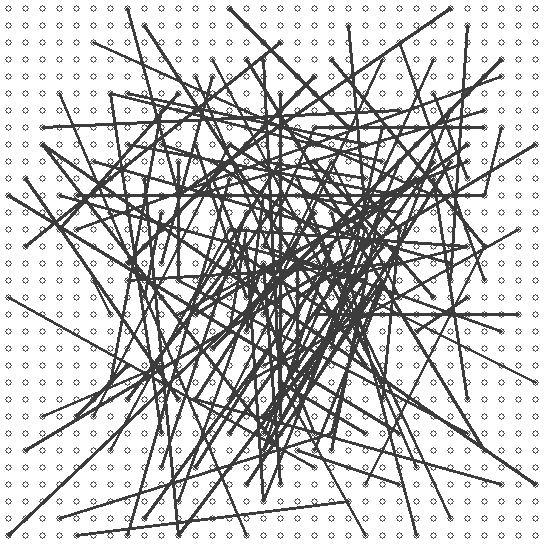
\includegraphics[width=0.25\linewidth]{brief-pattern}
	\caption{Salīdzināšanas pāri (parādīti 128 pāri)~\cite{BRIEF}.}
	\label{fig:pattern1}
\end{figure}
dod labus rezultātus.

Rublē~u.c.\cite{ORB} savukārt, lai kompensētu variances samazinājumu rBRIEF
deskriptoram, izmanto mašīnmācīšanās metodes, atlasot
salīdzināšanas pārus ar lielāko vērtības varianci un zemāko savstarpējo
korelāciju (sk.~\ref{sec:rbrief-def}~nod.).

BRIEF deskriptora aprēķināšanai, salīdzināmu deskriptoru kopas ietvaros
izmanto tos pašus salīdzināšanas pārus (matricas $\vb{a}$ un $\vb{b}$).
Tā kā šo pāru koordinātu punkti ir piesaistīti $\vb{p}$, un līdz ar to arī
attēla orientācijai, var viegli secināt, ka BRIEF nav rotācijas invariants.
Šo problēmu risina rBRIEF, kas apskatīts sekojošā apakšnodaļā.

\subsection{rBRIEF modifikācija} \label{sec:rbrief-def}
rBRIEF ir Rublē~u.c.\cite{ORB} izstrādāta rotācijas invarianta modifikācija
BRIEF deskriptoram, kura tiek izmantota par salāgošanas komponenti ORB
algoritmam. Idejas pamatā ir aprēķināt deskriptoru izmantojot
rotētas salīdzināšanas pāru punktu koordinātes, rotācijas leņķi nosakot pēc
raksturpunkta virziena komponentes (sk.~\ref{sec:ofast}~nod.).

Apzīmēsim rBRIEF deskriptoru ar $D_{n_d}$, kuru mēs varam definēt
pievienojot BRIEF $B_{n_d}$ rotācijas komponenti ar leņķi $\theta$:
\begin{equation}\label{eq:rbrief}
	D_{n_d}(\hat{\vb{p}}, \theta) := \sum_{i=1}^{n_d} 2^{i-1}
		\tau\left(\hat{\vb{p}},
		          \vb{R}(\theta) \times \vb{a}_i,
		          \vb{R}(\theta) \times \vb{b}_i\right)
\end{equation}
kur $\vb{R}(\theta)$ ir rotācijas matrica leņķim $\theta$, kas ir definēta kā:
\[
	\vb{R}(\theta) = 
		\begin{pmatrix}
			\cos\theta & -\sin\theta\\
			\sin\theta & \cos\theta
		\end{pmatrix}
\]

Uzdotā definīcija \eqref{eq:rbrief} ir idejiski ekvivalenta bet 
pierakstīta ievērojami citādāk nekā \cite{ORB} avotā, jo 
Rublē~u.c. visai liberāli reinterpretē mainīgo nozīmi.

Jānorāda, ka nodrošinot rotācijas invarianci, šī informācija tiek
,,atmesta'' no deskriptora, kas samazina tā varianci un tādējādi arī
tā diskriminitāti. Rublē~u.c.\cite{ORB}, šī samazinājuma kompensēšanai,
izstrādā mašīnmācīšanās metodes, ar kuru palīdzību tiek izvēlēti
salīdzināšanas pāri ar augstāko varianci. Izvēlētie punkti attēloti
\ref{fig:pattern2}a.~attēlā un ir novērojama salīdzināšanu pāru tendence
orientēties raksturpunkta rotācijas virzienā (attēlā virzienā uz augšu).
\begin{figure}[tbh]
	\centering
	\def\svgwidth{0.7\linewidth}
	{\input{img/rBRIEF.pdf_tex}}
	\caption{Mašīnmācīšanās metožu izvēlēti salīdzināšanas pāri
		(attēloti 64 pāri)~\cite{ORB}.}
	\label{fig:pattern2}
\end{figure}
Bet ir arī novērojams, ka izvēlētie pāri ir izvietoti līdzīgi, kas palielina
to savstarpējo korelāciju
un attiecīgi samazina to informatīvo vērtību. Rublē~u.c.\cite{ORB} izvēles
kritēriju papildina atlasot augstākās variances pārus, kuri atbilst
noteiktam korelācijas slieksnim (sk.~\ref{fig:pattern2}b.~att.), panākot
augstāku kopējo deskriptora diskriminitāti.

\subsection{Implementācijas modeļi}
\subsubsection{OpenCV algoritma implementācija} \label{sec:rbrief-ocv}
\TODO
